Finalmente, con cada una de las partes del prototipo debidamente conectadas y calibradas y la fuente de tritio debidamente situada y asegurada, únicamente nos resta exponer la  configuración de la parte electŕónica del sistema para empezar a medir la señal del prototipo. El objetivo es obtener un espectro energético de experimento con ayuda de un analizador multicanal analógico, MCA con tarjeta PCA3 y programa de adquisición Oxford WIN-MCA. La cadena electrónica   está basada en  tecnología NIM.

Necesitamos realizar una serie de transformaciónes a la señal para que, por un lado,  pueda ser analizada de manera adecuada por el MCA y, por otro lado, optimicemos al máximo la relación de la  señal sobre el fondo. El esquema electrónico utilizado se muestra en la figura~\ref{electronica}.

\begin{figure}[hbtp]
\centering
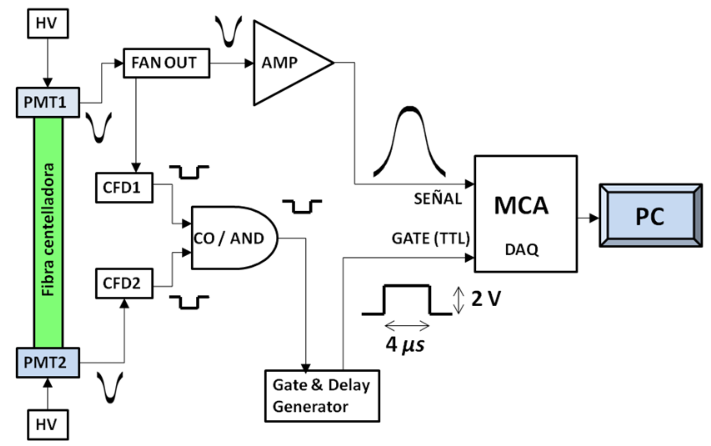
\includegraphics[scale=0.4]{Esquemaelectronico.png}
\caption{Esquema Electrico~\cite{Andres}\label{electronica}}
\end{figure}

 A continuación se procede a explicar el camino seguido por la señal y cada uno de los módulos que intervienen en estas transformaciones:

\begin{enumerate} 
\item{} En primer lugar sacaremos la señal de cada fotomultiplicador de la caja negra utilizada para apantallar la luz del exterior. Ello lo conseguimos con ayuda de cables BNC  ya que la caja dispone de puertos BNC macho que comunican el interior y el exterior.

\item {} Seguidamente dividimos la señales de un PMT en dos señales idénticas con ayuda de un divisor activo FAN IN/OUT. Esta no es una simple división de la señal donde se produce un reparto de la intensidad, sino una copia exacta de la señal de entrada. Necesitamos este típo de módulo y no una simple división ya que, como se explico al inicio del trabajo, la señal de tritio es una señal muy débil, por lo que no nos podemos permitir tener pérdidas ni divisiones de ésta. Esta división se ha realizado utilizando el módulo discriminador del cual hablaremos más adelante.

\item {} Ahora dividimos la señal en dos caminos. Por un lado una copia de la señal del PMT que se ha duplicado, se lleva a un preamplificador (marca Tennelec) y, seguidamente, a un amplificador (marca Tennelec, modelo TC 241) con una ganancia configurada de 50. Con este camino conseguimos amplificar de manera adecuada la señal de un PMT, del orden de $60~\milli\volt$ hasta un total de $3~\volt$, lo cual nos permite optimizar la escala disponible en el MCA (Entre 0 y $5~\volt$). Nos referiremos a la señal obtenida por este camino como señal 1.

\item{} Por otro lado, las dos señales restantes (una señal de cada PMT) es llevada por un camino distinto para obtener una señal que nos indique cuando hay coincidencia. Para conseguir esta segunda señal hay que tener en cuenta que los PMTs ofrecen señales analógicas y negativas. Por tanto, dado que esta señal de coincidencia será creada y tratada con tecnología NIM, necesitamos convertir estas señales en señales lógicas de estándar NIM. 

Esto lo conseguimos pasando cada una de estas dos señales por un módulo discriminador (CAEN, de cuatro canales). Este ofrece una señal lógica en forma de escalón negativo de altura $800~\milli\volt$ y anchura variable, en nuestro caso $30~\ns$, para cada una de las señales, siempre y cuando la señal de entrada asociada supere un umbral determinado, en nuestro caso $30~\milli\volt$ (hablamos en valores absolutos, hay que tener en cuenta que estas son negativas). De esta forma eliminamos de manera considerable la corriente oscura de los PMT y, por extensión, el fondo.

\item{} A continuación hacemos pasar ambas señales de la salida del discriminador por un módulo de coincidencias modelos CERN N 6234. Este genera una señal de salida  sólo si las dos señales de entrada (procedentes de cada PMT tras pasar por el discriminador) están en coincidencia temporal. 

Estas cuatro señales (PMT, puerta lógica de cada PMT y puerta lógica de coincidencia) pueden verse en la figura~\ref{señales}:

\begin{figure}[hbtp]
\centering
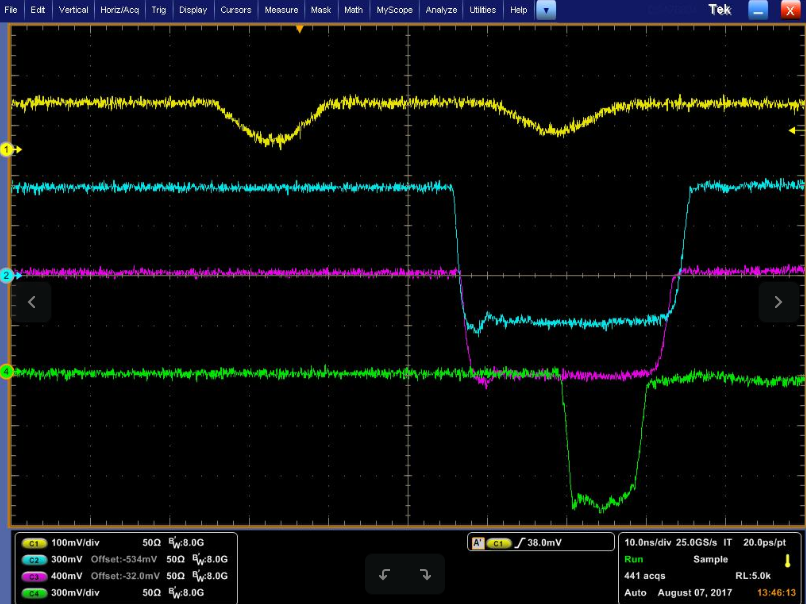
\includegraphics[scale=0.4]{SenalesNIM.png}
\caption{ Señal de salida del PMT (1), señal de salida del discriminador para cada PMT (2 y 3) y señal de salida del módulo de concidencias respectivamente\label{señales}}
\end{figure}


\item {} Luego pasamos esta señal de coincidencia a un módulo Gate \& Delay Generator (marca ORTEC, modelo 416A). Este módulo nos genera una señal lógica en forma de escalón positivo, de altura $2~\volt$ y anchura de $4~\mu s$, anchura suficiente para comprender en su interior la totalidad de la señal 1. Esta puerta debe ser positiva debido a que este es un requisito del MCA. Además aplicaremos un retraso a esta señal que compense la diferencia de caminos seguidos entre esta y la señal 1. Nos referiremos a la señal obtenida por este camino como señal 2.

\item {} En último lugar pasamos al MCA tanto la señal 1 (señal de un PMT amplificada) como la señal 2 (que nos indica cuando ambos fotomultiplicadores han detectado en coincidencia). Estas dos señales pueden verse en la  figura~\ref{señales MCA}.

\begin{figure}[hbtp]
\centering
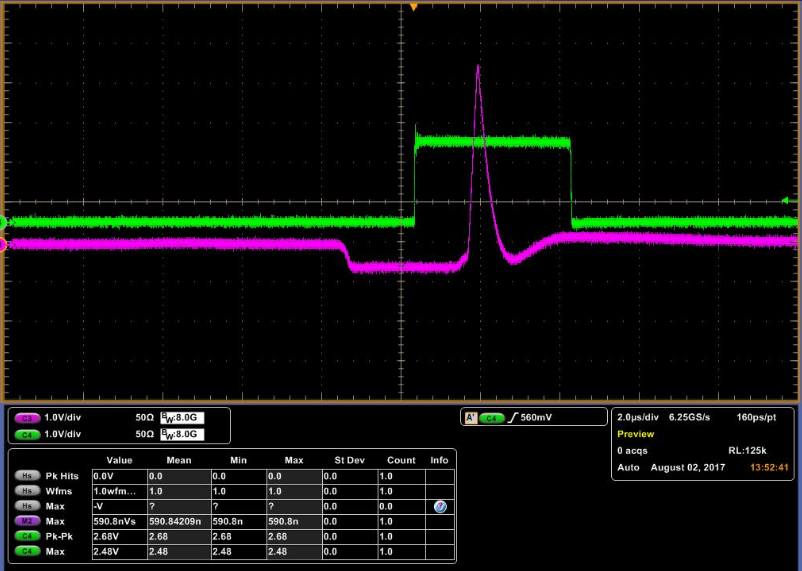
\includegraphics[scale=0.4]{SenalesMCA.png}
\caption{Señales de entrada del MCA\label{señales MCA}}
\end{figure}


El MCA  empleado dispone de la opción de crear un histograma de  la señal 1, la cual sólo  se leerá si la señal 2 es no nula, es decir, sólo leera la señal 1 en la ventana proporcionada por la señal 2. Aquí reside la importancia de ajustar bien la anchura de la señal 2 ya que, debe de ser suficiente para contener en todo momento la señal 1 pero ajustada tanto como sea posible para evitar la entrada de corriente oscura.

Con esto conseguimos realizar una detección en coincidencia de ambos fotomultiplicadores, lo cual nos reducirá enormemente el fondo del experimento.

\end{enumerate}



